% !TEX root = base-r.tex

\begin{block}{Timeline}
Fill in the blanks with your target deadlines. If a particular step does not apply to your work, feel free to cross it out. 
\begin{table}[]
\Large
\color{darkgray}
\begin{tabular}{rlll}
\multicolumn{1}{c}{\textcolor{headercolor}{\textbf{TIMELINE}}} & \multicolumn{2}{c}{\textcolor{headercolor}{\textbf{YOUR ACTION ITEMS}}} & \textcolor{headercolor}{\textbf{RESOURCES}}\\
& & & \\
\multirow{2}{*}{\color{violet}\framebox(80, 25){} $\cdots$\makebox[0pt][c]{$\bullet$}}  &\multirow{2}{*}{\textbf{Ethics Approval}} &  $\cdot$ collect data sharing & [Check your universities guidelines]\\
 & & consent& \\
 %& & & \\
\multirow{2}{*}{\color{violet}\framebox(80, 25){} $\cdots$\makebox[0pt][c]{$\bullet$}} & \multirow{2}{*}{\textbf{Preregistration}} & Check if a Preregistration could be beneficial for your work. &
    \href{https://aspredicted.org/}{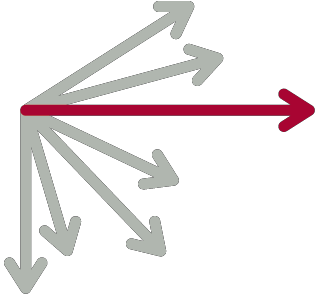
\includegraphics[width=0.8cm]{base-r/img/aspredicted_penn_wharton.png}}  
\href{https://aspredicted.org/}{AsPredicted.org}\\
 & & If yes, Preregister & \href{https://osf.io/registries}{
\includegraphics[width=0.8cm]{base-r/img/osf registries.png}}  
\href{https://help.osf.io/article/345-create-registrations}{OSF Guide and templates}  \\
  & & & \\
  \multirow{2}{*}{\color{violet}\framebox(80, 25){} $\cdots$\makebox[0pt][c]{$\bullet$}} &\textbf{Data Collection} &  $\cdot$ deidentify/anonymize data, &  \href{https://edps.europa.eu/system/files/2021-04/21-04-27_aepd-edps_anonymisation_en_5.pdf}{
\includegraphics[width=0.75cm]{base-r/img/anonymise_data.png}} 
  \href{https://edps.europa.eu/system/files/2021-04/21-04-27_aepd-edps_anonymisation_en_5.pdf}{How To}\\
 \color{violet} & \textbf{and Organization} & choose a non-proprietary file format (e.g., csv) &  \\
 & &$\cdot$ create a data dictionary & \href{https://github.com/yvonnejansen/posture/blob/master/data/exp1_column-description.csv}{
\includegraphics[width=0.75cm]{base-r/img/data_dictionary.png}} \href{https://github.com/yvonnejansen/posture/blob/master/data/exp1_column-description.csv}{Check Example}\\
  & & & \\
\multirow{2}{*}{\color{violet}\framebox(80, 25){} $\cdots$\makebox[0pt][c]{$\bullet$}} &\textbf{Data Analysis} &  $\cdot$ clean, executable, and & \href{https://www.r-project.org/}{
\includegraphics[width=0.95cm]{base-r/img/Rlogo.png}}  \href{https://www.r-project.org/}{R} \quad \href{https://www.python.org/}{
\includegraphics[width=0.75cm]{base-r/img/python_logo.jpg}}  \href{https://www.python.org/}{Python} \quad \href{ https://jasp-stats.org/}{
\includegraphics[width=0.8cm]{base-r/img/JASP_logo.png}}  \href{ https://jasp-stats.org/}{JASP}\\
 & & commented code/script & \\
 & & &  \\
%  & & & \\
\multirow{2}{*}{\color{violet}\framebox(80, 25){} $\cdots$\makebox[0pt][c]{$\bullet$}} &\textbf{Supplementary} &  Add to a repository: &  \href{https://zenodo.org/}{
\includegraphics[width=1.5cm]{base-r/img/zenodo.png}}  \href{https://zenodo.org/}{Zenodo.org}\\
 & \textbf{Material} & $\cdot$ data,  &
 \href{https://dataverse.harvard.edu/}{
\includegraphics[width=1.5cm]{base-r/img/harvard_dataverse.png}} \href{https://dataverse.harvard.edu/}{Harvard Dataverse}\\
  & & $\cdot$ study protocols,  & \href{https://osf.io/}{
\includegraphics[width=0.8cm]{base-r/img/osf registries.png}}   \href{https://osf.io/}{OSF Repository}\\
 & & $\cdot$ analysis scripts, &
  \href{https://github.com/}{
\includegraphics[width=0.8cm]{base-r/img/GitHub-Mark-64px.png}} \href{https://github.com/}{GitHub}
  \\ %\href{https://www.icpsr.umich.edu/web/pages/}{ICPSR}
  & & $\cdot$ videos, and &  \href{https://gitlab.com/}{
\includegraphics[width=0.8cm]{base-r/img/gitlab-logo-500.png}} \href{https://gitlab.com/}{GitLab}\\
& & $\cdot$ anything else relevant to you. & \\
& & & \\
\multirow{2}{*}{\color{violet}\framebox(80, 25){} $\cdots$\makebox[0pt][c]{\faTrophy}} & &  &\\
& \multicolumn{2}{c}{
\includegraphics[width=0.75cm]{base-r/img/star (1).png} \color{violet}YOU DID IT! 
\includegraphics[width=0.75cm]{base-r/img/star (1).png}}& \\
\end{tabular}
\end{table}



% \begin{table}
% %\caption{Fill in the blanks with your target deadlines}
% \centering
% \begin{minipage}[t]{.99\linewidth}
% \color{gray}
% \rule{\linewidth}{1pt}
% \ytl{\framebox(60,20){}}{Include Data Sharing Statement in the Ethics Approval}
% \ytl{\framebox(60,20){}}{Preregistration}
% \ytl{\framebox(60,20){}}{Data Collection and Organization}
% \ytl{\framebox(60,20){}}{Deidentification of Participant Data}
% \ytl{\framebox(60,20){}}{Create a Data Dictionary}
% \ytl{\framebox(60,20){}}{Analyse Data}
% \ytl{\framebox(60,20){}}{Clearly Commented Code}
% \ytl{\framebox(60,20){}}{Submit data to a FAIR repository}
% \ytl{\framebox(60,20){}}{Submit supplementary material to a repository}
% \bigskip
% \rule{\linewidth}{1pt}%
% \end{minipage}%
% \end{table}

\end{block}
